\documentclass[12pt,a4paper]{article}
\usepackage{xeCJK}
\usepackage{fontspec}
\setmainfont{Times New Roman}
\setCJKmainfont{PingFang TC}
\usepackage[colorlinks=true, urlcolor=blue, linkcolor=red]{hyperref}
\usepackage{amsmath, amsfonts, amssymb, amsthm, algorithm, booktabs, listings}
\DeclareMathAlphabet{\mathbbold}{U}{bbold}{m}{n}
\usepackage[dvipsnames,usenames]{xcolor}
\usepackage[noend]{algpseudocode}
\usepackage{tikz}
\usepackage{fancyhdr}
\usepackage{geometry}
\newgeometry{top=2cm, bottom=2cm, left=1.5cm, right=1.5cm}
\usepackage[shortlabels]{enumitem}
\usepackage{cleveref}
\usepackage{mdframed}
\usepackage[most]{tcolorbox}
\hypersetup{citecolor=blue}
\usepackage{subcaption}
\theoremstyle{definition}
\newtheorem{definition}{Definition}[subsection]
\newtheorem{statement}{Statement}[subsection]
\newtheorem{theorem}{Theorem}
\newtheorem{lemma}[theorem]{Lemma}
\newtheorem{claim}[theorem]{Claim}
\usepackage[backend=biber,style=alphabetic,sorting=ynt]{biblatex}
\hypersetup{linkcolor=black}
\addbibresource{references.bib}
\pagestyle{fancy}

\input{shun4colors}
\newcommand{\bs}{\textbackslash}
\newcommand{\boxtxt}[1]{\boxed{\text{#1}}}
\newcommand{\op}[1]{\operatorname{#1}}
\newcommand{\OPT}{\mathrm{OPT}}

\tcbuselibrary{listings}
\newtcblisting{shuncode}[1][]{
  listing only,
  listing options={
      language=C,
      basicstyle=\ttfamily\small,
      keywordstyle=\color{blue},
      commentstyle=\color{green!50!black},
      stringstyle=\color{red}
  },
  colframe=cyan!80!black,
  colback=cyan!10,
  title={#1},
  enhanced,
}

\newtcblisting{shuncmd}[1][]{
  listing only,
  listing options={
    language=bash,
    basicstyle=\ttfamily\small,
    keywordstyle=\color{blue},
    commentstyle=\color{green!50!black},
    stringstyle=\color{red},
    breaklines=true
  },
  colframe=cyan!80!black,
  colback=cyan!10,
  title={#1},
  enhanced,
}

\newcommand{\shunsc}[1]{%
  \textsf{\textsc{#1}}
}

\newcommand{\shuncal}[1]{%
  \mathsf{\mathcal{#1}}
}

\newcommand{\hn}{
  \vspace{0.5em}
}

\newcommand{\nl}{
  \vspace{1.0em}
}

\lhead{Principles of Microeconomics}
\chead{Terminology and Key Points}
\rhead{Shun (@shun4midx)}

\begin{document}
\begin{center}
  {\Large \bf Principles of Microeconomics Terminology and Key Points}\\[8pt]
  \textbf{Author:} Shun (@shun4midx)
\end{center}

\bluesec{Chapter 1: Ten Principles of Economics}

\purplesec{Ten Principles of Economics}
\noindent \hlbf{How People Make Decisions} \\
\begin{enumerate}
    \item People face trade-offs
    \item The cost of something is what you give up to get it
    \item Rational people think at the margin
    \item People respond to incentives
    
    \medskip
    \hspace{-\leftmargin}\noindent\hlbf{How People Interact}
    \medskip
    \item Trade can make everyone better off
    \item Markets are usually a good way to organize economic activity
    \item Governments can sometimes improve market outcomes
    
    \medskip
    \hspace{-\leftmargin}\noindent\hlbf{How the Economy as a Whole Works}
    \medskip
    \item A country's standard of living depends on its ability to produce goods and services
    \item Prices rise when the government prints too much money
    \item Society faces a short-run trade-off between inflation and unemployment
\end{enumerate}

\purplesec{What is Economics?}
\begin{itemize}
    \item \textbf{Scarcity}: The limited nature of society's resources
    \item \textbf{Economics}: The study of how society manages its scarce resources
\end{itemize}

\purplesec{How People Make Decisions}
\begin{itemize}
    \item \textbf{Efficiency}: The property of society getting the most it can from its scarce resources.
    \item \textbf{Equality}: The property of distributing economic prosperity uniformly among the members of society
    \item \textbf{Opportunity cost}: Whatever must be \textbf{given up} to obtain that item
    \item \textbf{Rational people}: People who systematically do the best they can to achieve their objectives, given the opportunities available to them
    \item \textbf{Marginal change}: A small \textbf{incremental adjustment} to an existing plan of action
    \item \textbf{Incentive}: Something that induces a person to act, such as a \textit{punishment or a reward}
    \item \textbf{Sunk cost}: Cost that is gone \textbf{regardless of what's decided next}
\end{itemize}

\purplesec{How People Interact}
\begin{itemize}
    \item \textbf{Market economy}: An economy that allocates resources through the \textbf{decentralized decisions} of many firms and households as they \textbf{interact in markets} for goods and services
    \item \textbf{Adam Smith's Invisible Hand} steers markets and households towards outcomes that maximize the well-being of society as a whole
    \item \textbf{Property rights} are the ability of an individual to \textbf{own and exercise control} over scarce resources
    \item \textbf{Market failure} is a situation in which a market left on its own \textbf{fails to allocate resources efficiently}
    \item \textbf{Externality}: The effect of one person's actions on a bystander (e.g. pollution)
    \item \textbf{Market power}: A single actor's ability to influence market prices (e.g. monopoly)
\end{itemize}

\purplesec{How the Economy as a Whole Works}
\begin{itemize}
    \item \textbf{Productivity} is the \textbf{quantity of goods and service} produced from \textbf{each unit} of labor input
    \item \textbf{Inflation} is an \textbf{increase in the overall level of prices} in the economy
    \item \textbf{The business cycle} refers to fluctuations in economic activity, such as employment and production
\end{itemize}

\newpage

\bluesec{Chapter 2: Thinking Like an Economist}

\purplesec{The Economist as a Scientist}

\begin{itemize}
    \item A \textbf{natural experiment} is a real-world event that, by chance, \textbf{exposes one group to change} while leaving a similar \textbf{comparison group} unaffected, creating something close to a controlled experiment.
\end{itemize}

\purplesec{The Circular-Flow Diagram}

\begin{itemize}
    \item The \textbf{Circular-Flow Diagram} is a visual model of the economy that shows how dollars flow through markets among households and firms. It \hlbf{leaves out government and international trade.}
\end{itemize}

\begin{figure}[h]
    \centering
    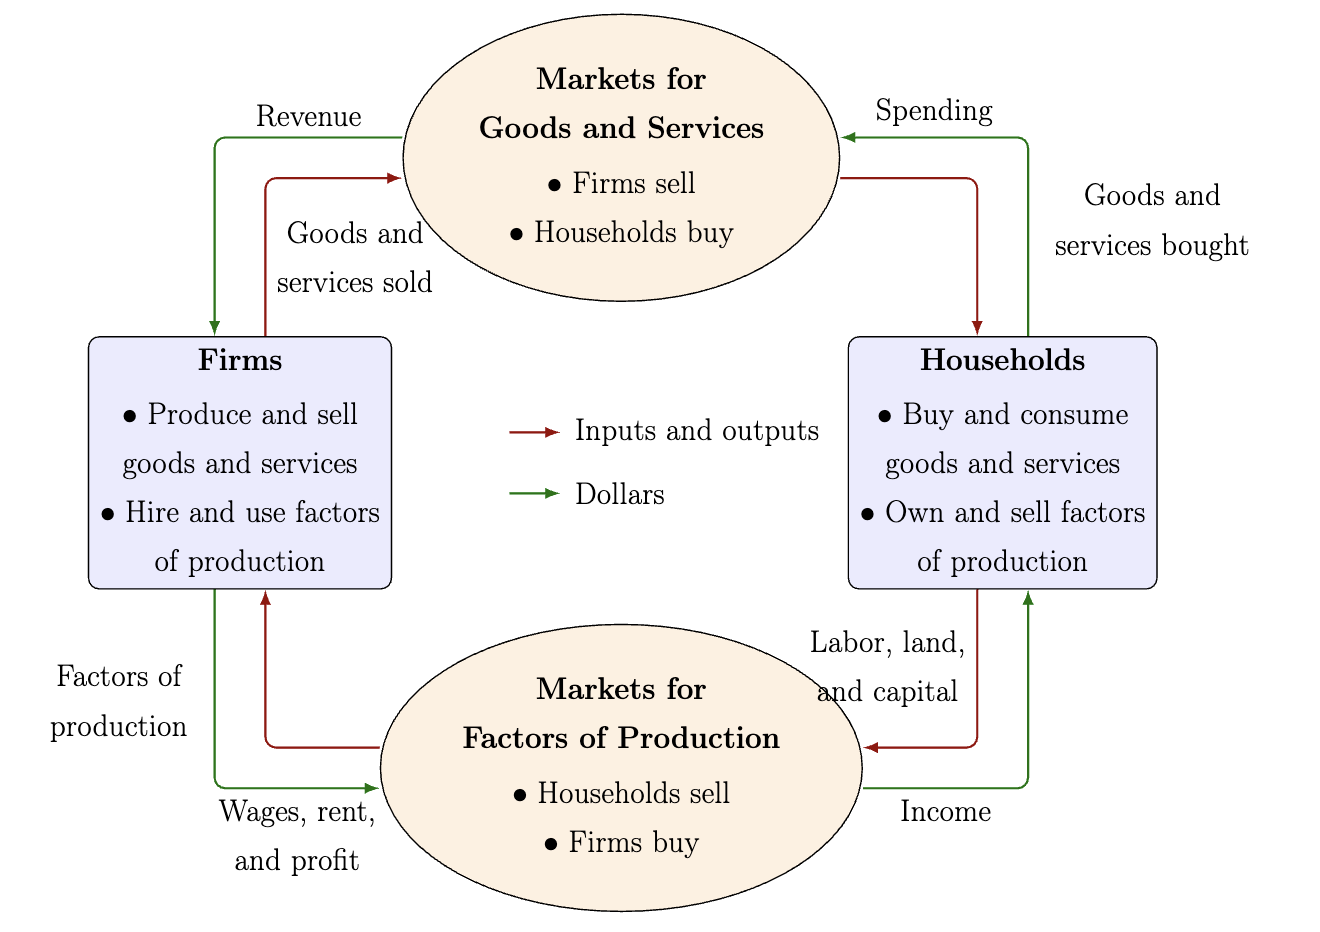
\includegraphics[width=0.85\textwidth]{imgs/circular_flow_diagram.png}
    \caption{The circular-flow diagram}
    \label{fig:circular_flow_diagram}
\end{figure}

\purplesec{The Production Possibilities Frontier}

\begin{itemize}
    \item \textbf{Production Possibilities Frontier (PPF)}: A graph that shows the various combinations of output that an economy can produce, given its available factors of production and technology.
    \item An outcome is \textbf{efficient} if the economy is getting all it can from its scarce resources: \textbf{no more of one good can be produced} without producing less of the other
    \item An outcome is \textbf{infeasible} if the current resources the economy has \textbf{are not enough} to produce the desired goods
    \item An outcome is \textbf{inefficient} if the economy can \textbf{still produce more goods} with its current resources
\end{itemize}

\purplesec{Microeconomics and Macroeconomics}

\begin{itemize}
    \item \textbf{Microeconomics}: The study of how \textbf{households and firms} make decisions and how they interact in \textbf{specific markets}
    \item \textbf{Macroeconomics}: The study of \textbf{economy-wide} phenomena, such as inflation, unemployment, and economic growth
\end{itemize}

\purplesec{Positive vs Normative Statements}

\begin{itemize}
    \item \textbf{Positive statements} are \textit{descriptive}, and attempt to describe the world \textbf{as it is}. In principle, they can be confirmed or refuted with evidence
    \item \textbf{Normative statements} are \textit{perscriptive}, and attempt to describe how the world \textbf{ought to be}, and cannot be settled by evidence alone.
\end{itemize}

\newpage

\bluesec{Chapter 3: Interdependence and the Gains from Trade}

\begin{itemize}
    \item \textbf{Interdependence} refers to how we \textbf{rely on people all over the world} to provide us with goods, and in return provide something they want.
    \item \textbf{Absolute advantage} is the ability to produce a good using \textbf{fewer inputs} than another producer.
    \item \textbf{Comparative advantage} is the ability to produce a good at a \textbf{lower opportunity cost} than another producer.
    \item \textbf{Imports} are goods produced abroad and sold domestically
    \item \textbf{Exports} are goods produced domestically and sold abroad
\end{itemize}

\newpage

\bluesec{[INCOMPLETE] Chapter 4: Market Forces of Supply and Demand}

\purplesec{Markets and Competition}

\begin{itemize}
    \item A \textbf{market} is a \textbf{group of buyers and sellers} of a particular good or service
    \item A \textbf{competitive market} is a market with \textbf{so many} buyers and sellers that each one has a \textbf{negligible impact} on the market price
    \item A \textbf{monopoly} is a market with a \textbf{single seller}, who \textbf{sets the price} rather han taking it as given
\end{itemize}

\purplesec{Demand}

\begin{itemize}
    \item The \textbf{quantity demanded} of a good is the amount that buyers are \textbf{willing and able to purchase}
    \item The \textbf{law of demand} states that, other things being equal, the \textbf{quantity demanded} of a good \textbf{falls} when the \textbf{price} of the good \textbf{rises}
    \item A \textbf{demand schedule} is a \textbf{table} showing the \textbf{relationship between the price of a good and the quantity demanded}, holding everything else constant
    \item A \textbf{demand curve} is a \textbf{graph} of the relationship between the price of a good and the quantity demanded
    \item \textbf{Market demand} is the \textbf{sum of the individual demands} of every buyer in the market, and the market demand curve is found by adding the individual curves horizontally
\end{itemize}

\purplesec{Factors that Shift a Demand Curve}

\begin{itemize}
    \item Income
    \item Prices of related goods
    \item Tastes
    \item Expectations
    \item Number of buyers
\end{itemize}

\purplesec{Normal and Inferior Goods}

\begin{itemize}
    \item A \textbf{normal good} is one for which \textbf{demand rises when income rises}
    \item A \textbf{inferior good} is one for which \textbf{demand falls when income rises}
\end{itemize}

\end{document}